\documentclass[12pt,a4paper]{article}
\usepackage[a4paper,margin=3cm]{geometry}

% Turns off all hyphenation in document
\usepackage[none]{hyphenat}

% Turn off page numbering (on pages other than first one)
\pagestyle{empty}

% Fonts and symbols
\usepackage{textcomp}
\usepackage{tgpagella}
\usepackage{amsthm}

% No indent before itemizes
\usepackage{enumitem}
\setlist[itemize]{leftmargin=*}
\setlist[description]{leftmargin=*}

% Decrease/control white space above title
\usepackage{titling}
\setlength{\droptitle}{-2cm}

% Control length to left of table column
\setlength{\tabcolsep}{0em}
% Control length between paragraphs
\setlength{\parskip}{10pt}

% Email addresses as hyperlinks (via `\mailto')
\usepackage{hyperref}
\hypersetup{colorlinks,urlcolor=blue}
\usepackage{url}
\newcommand{\mailto}[1]{\href{mailto:#1}{\url{#1}} }

\usepackage{pdfpages}

\newcommand{\CPP}
{C\nolinebreak[4]\hspace{-.05em}\raisebox{.22ex}{\footnotesize\bf ++ }}

% A labelled list (basically an array of rows with form LABEL ITEM)
\newenvironment{llist}
	{\renewcommand{\arraystretch}{1.5}\begin{tabular}{p{3cm} p{12cm}}}
	{\end{tabular}}

%% Date settings for \today
\usepackage{datetime}
% Declare a new date format
\newdateformat{monthyear}{\monthname[\THEMONTH] \THEYEAR}
% Indicate that we should actually _use_ this format for \today
\monthyear

\title{\bfseries \huge Rob Cornish}
% XXX: Really should be \subtitle, but no easy way to do this..
\author{Curriculum Vit\ae}
\date{\today}

\begin{document}
\maketitle

% Suppress page numbering on first page
\thispagestyle{empty}
% Control space between title and first sect2010-2011 Swimmingion
%%\vspace{3em}

\section*{Contact details}
\begin{llist}
	\textit{Full name} & John Robert Macaulay Cornish \\
	\textit{Address} & 19 Bath Rd, Glen Iris, VIC, 3146 \\
	\textit{Date of Birth} & 23rd January, 1992 \\
	\textit{Telephone} & H: 03 9809 0134 \newline M: 0409 331 882 \\
	\textit{Email} & \texttt{j.cornish@student.unimelb.edu.au}
\end{llist}

\section*{Education}
\begin{llist}
	2012-present & Transferred to Bachelor of Science, University of Melbourne, majoring in Electrical Systems. Completion planned for 2013. \\
	2011-present & Diploma of Mathematical Sciences, University of Melbourne, majoring in Pure Mathematics \\
	2010-2012 & Commenced Bachelor of Arts, University of Melbourne, majoring in Philosophy and History and Philosophy of Science \\
	2009 & VCE ENTER score of 99.55 \\
\end{llist}

\section*{Academic awards and achievements}
\begin{llist}
  2013 & Selected for CSIRO (QLD) Computational Infomatics Vacation Scholarship
         program \textit{(Accepted)} \newline \newline
         Selected for CSIRO (NSW) Astronomy and Space Science Vacation
         Scholarship program \textit{(Declined)}\newline \newline
         Selected for the Melbourne University Department of Mathematics and
         Statistics' Vacation Scholarship program \textit{(Declined)} \newline \newline
         Winner of MUECC SumoRobo Competition \\
	2012 & Faculty of Arts Dean's Honours List for 2011 \newline \newline
         Selected for the Melbourne School of Engineering's Summer Research
         Experience program \textit{(Accepted)} \newline \newline
         Selected for the Melbourne University Department of Mathematics and
         Statistics' Vacation Scholarship program \textit{(Declined)} \\
	2011 & Hastie Exhibition for ``highest overall results in two Philosophy subjects''
\end{llist}

%\newpage
%\vspace{6em}
\section*{Employment}
\begin{llist}
  2012-2013 & Research assistant with Optimization and Programming Languages
  Research Group (University of Melbourne). Main research topic: a program
  transformation for array manipulating programs. \\
	2011-present & Lifeguard, Ashburton Pool and Recreation Center \\
	2010-2011 & Swimming instructor, Ashburton Pool and Recreation Center \\
\end{llist}

\section*{Computer Skills}
\begin{itemize}
  \item Strong programming skills in C/\CPP, Python, Ruby, Bash, MATLAB,
    Perl. Working knowledge of Lisp, Javascript, PHP. 
	\item Proficient with {\LaTeX} and XML/HTML.
  \item Proficient with Unix command-line environment (Arch Linux user).
  \item Proficient with using version control tools (Git and Subversion in
    particular).
\end{itemize}

\section*{References}
Please find submitted letters of recommendation from the following individuals: \\ \\

\noindent
A/Prof. Harald S\o ndergaard  \\
Department of Computing and Information Systems \\
The University of Melbourne \\
Email: \mailto{harald@unimelb.edu.au} \\

\noindent
A/Prof. Jan De Gier \\
Department of Mathematics and Statistics\\
The University of Melbourne \\
Email: \mailto{jdgier@unimelb.edu.au} \\

\noindent
A/Prof. Michael Cantoni \\
Department of Electrical and Electronic Engineering \\
The University of Melbourne \\
Email: \mailto{cantoni@unimelb.edu.au}

\hfill \qedsymbol

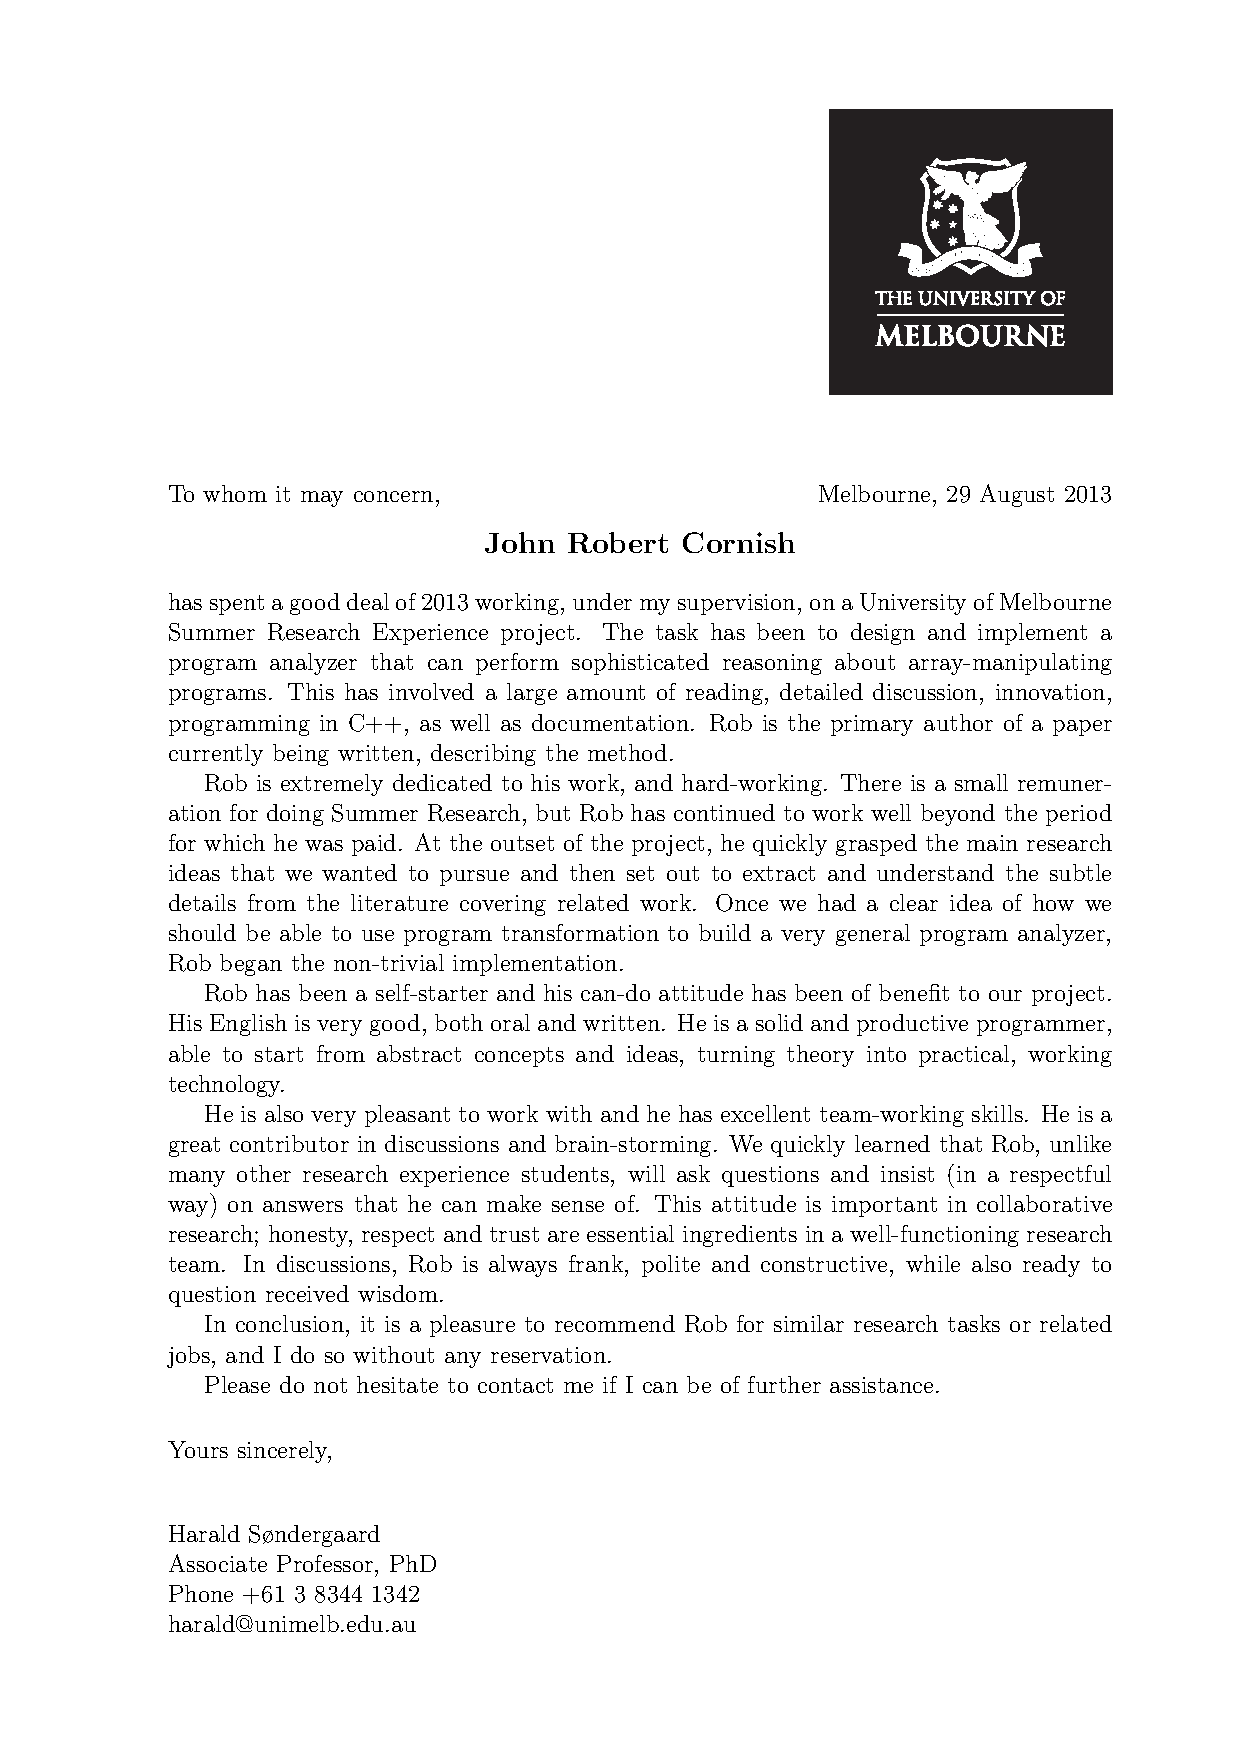
\includepdf[turn=false,pages=-]{pdf/reference_sondergaard.pdf}

\includepdf[turn=false,pages=-]{pdf/reference_de_gier.pdf}

\includepdf[turn=false,pages=-]{pdf/reference_cantoni_csiro.pdf}
%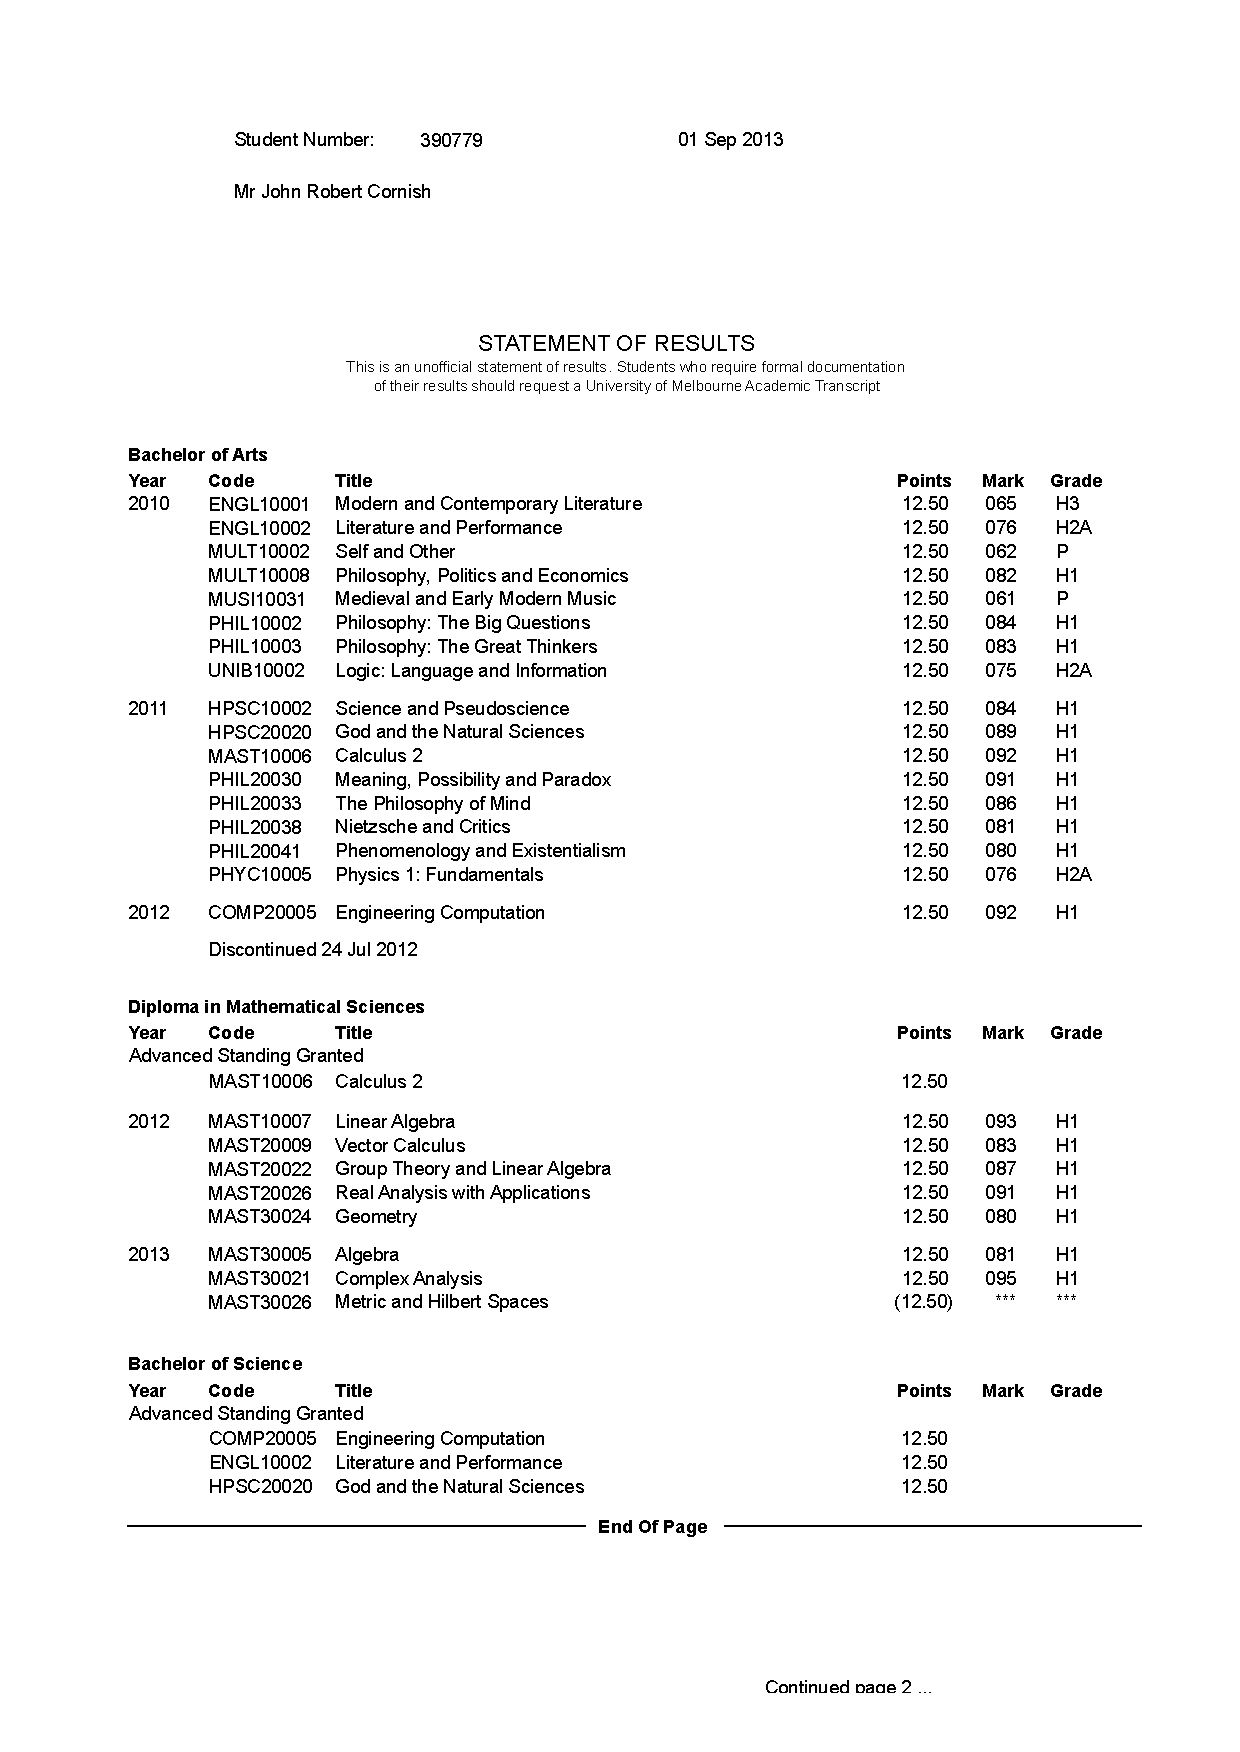
\includepdf[nup=1x2,turn=false,landscape=true,pages=-]{pdf/AcademicRecord-390779-01_Sep_2013.pdf}

\end{document}
